\section{Theorie}
\label{sec:Theorie}
\subsection{Einleitung}
Im folgenden Experiment soll das Trägheitsmoment dreier unterschiedlicher Körper bestimmt werden.
Zusätzlich wird ein Körper verwendet, welcher seine Geometrie verändern kann, aber seine Masse beibehält,
wodurch geometrische Beziehungen zum Trägheitsmoment untersucht werden können.

\subsection{Trägheitsmoment \footnote{Unter Verwendung der Quellen \cite{taschenbuch}, \cite{Versuchsanleitung}}}
Analog zur Masse in der Translation wird für Rotationsbewegungen das Massenträgheitsmoment $\symup{I}$ verwendet.
Für eine vollständige Beschreibung der Rotationsdynamik werden zusätzlich die Winkelbeschleunigung $\dot{\omega}$
und das Drehmoment $\symup{M}$ benötigt. Letzteres ist das Äquivalent der Kraft $\symup{F}$ in der Translation.
Im Vergleich wird die Beziehung deutlich
\begin{equation}
    \label{eqn:FmaAnalogie}
    F = m a \quad ,\quad M = I\dot{\omega} \:.
\end{equation}
Dabei gilt für das Massenträgheitsmoment
\begin{equation*}
    I = \sum_i \Delta m_i r_i^2
\end{equation*}
für diskrete und
\begin{equation}
    \label{eqn:integralInertia}
    I = \int r^2 dm
\end{equation}
für infinitesimale Massen.

Da sich \eqref{eqn:integralInertia} aus den Massenabständen bezüglich einer Drehachse errechnet,
ist die Bestimmung für einfache Geometrien nicht aufwendig und meist in Formelsammlungen zu finden.
Bei komplexeren Körpern jedoch ist dies nicht mehr der Fall, sodass dieser mit den einfacheren Geometrien
approximiert wird.
Hilfreiche Referenzen sind Zylinder, dünne, lange Stäbe, Kugeln, Quader und Hohlzylinder, wobei Stäbe und Hohlzylinder
Spezialfälle eines Zylinders darstellen.
\begin{figure}
    \centering
    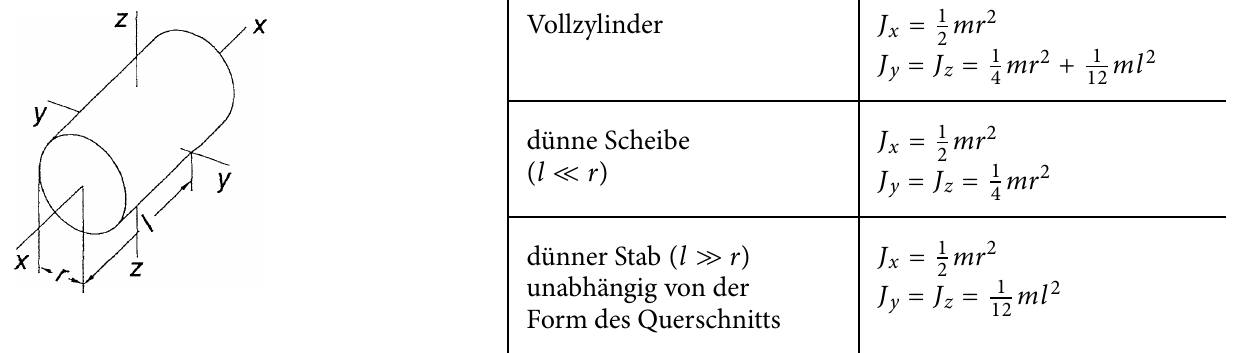
\includegraphics[width=0.9\textwidth]{plots/TrägheitZylinder.png}
    \caption{Das Massenträgheitsmoment eines Zylinders.\cite{taschenbuch}}
    \label{fig:traegZyl}
\end{figure}

\begin{figure}
    \centering
    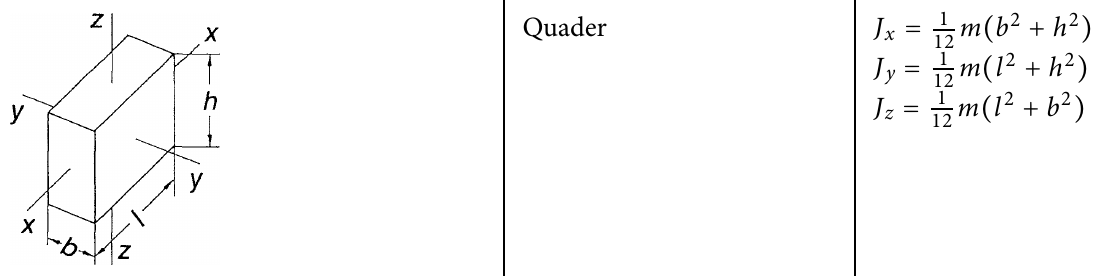
\includegraphics[width=0.9\textwidth]{plots/TrägheitQuader.png}
    \caption{Das Massenträgheitsmoment eines Quaders.\cite{taschenbuch}}
    \label{fig:traegQuader}
\end{figure}

\begin{figure}
    \centering
    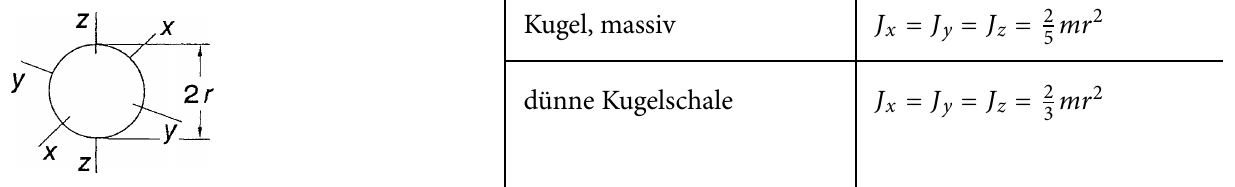
\includegraphics[width=0.9\textwidth]{plots/TrägheitKugel.png}
    \caption{Das Massenträgheitsmoment einer Kugel.\cite{taschenbuch}}
    \label{fig:traegKug}
\end{figure}

In den Abbildungen gilt $J \equiv I$.

Es ist nicht immer der Fall, dass die Rotationsachse auch eine der oben angezeigten Körperachsen entspricht.
Um das Massenträgheitsmoment dennoch ohne aufwendige Integration bestimmen zu können, wird der \textit{Steiner'sche
Satz} angewendet. Wenn $I$ für eine der Trägheitsachsen bekannt ist, wird der gesamte Körper parallel
zu dieser Achse verschoben und mit der Gleichung
\begin{equation}
    I = I_U + ma^2
\end{equation}
berechnet. Hier entspricht $I_U$ dem ursprünglichen Massenträgheitsmoment und $a$ dem Abstand zur Achse, um die 
parallel verschoben wird.

\subsection{Winkelrichtgröße}
Das Direktionsmoment $D$, auch Winkelrichtgröße genannt, entspricht analog der Federkonstanten bei longitudinalen Auslenkungen. Das Moment ist also
die Proportionalitätskonstante bei einer mechanischen Torsion zwischen dem Drehwinkel $\vec{\varphi}$ und dem Drehmoment $\vec{M}$
\begin{equation}
    \label{eqn:FederAnalogie}
    \vec{M} = D\cdot \vec{\varphi} \qquad , \qquad \vec{F} = k\cdot \vec{s}\:.
\end{equation}
Zudem gilt die Beziehung 
\begin{equation}
    \label{eqn:DrehKraft}
    \vec{M} = \vec{F} \times \vec{r}\:,
\end{equation}
wobei $\vec{F}$ einer angreifenden Kraft auf den drehbaren Körper bei dem Abstand $\vec{r}$ entspricht.


Das Drehmoment $M$ ist bei Spiralfedern eine lineare Funktion der Auslenkung $\varphi$ mit dem Konstanten Vorfaktor $D$.
Es stellt also eine rücktreibende Kraft dar, die auf den drehbaren Körper wirkt.
Durch die lineare Natur des Drehmoments entspricht die Dynamik die einer harmonischen Schwingung bei vorhandener Auslenkung.
Die bei realen Schwingern vorhandene Dämpfung wird für diesen Versuch nicht berücksichtig.

Die ungedämpfte Eigenkreisfrequenz einer harmonischen, longitudinalen Federschwingung wird vorausgesetzt als 
\begin{equation*}
    \omega = \frac{2\pi}{T} = \sqrt{\frac{k}{m}}\:.
\end{equation*}

Durch die in \eqref{eqn:FmaAnalogie} gezeigte Analogie ergibt\footnote{In realen Fällen muss beachtet werden, dass die Drillachse ein eigenes Trägeheitsmoment $I_D$ besitzt, welches für genaue Berechnungen zuerst bestimmt werden muss.} sich dann für $T$

\begin{alignat}{2}
    &       & \omega    & = \frac{2\pi}{T} = \sqrt{\frac{D}{I}}  \\
    & \iff  & T         & = 2\pi \sqrt{\frac{I}{D}}\:.
    \label{eqn:SchwingFeder}
\end{alignat}

Das Direktionsmoment $D$ wird in einer \textit{statischen Methode} durch Messung der Auslenkung $\varphi$ als Funktion der Kraft $F$ mit \eqref{eqn:DrehKraft} und \eqref{eqn:FederAnalogie}
berechnet. Ist das Massenträgheitsmoment $I$ bekannt, wird $D$ in einer \textit{dynamischen Methode} durch Messung der Schwingungsdauer $T$ mit \eqref{eqn:SchwingFeder}
bestimmt.

\subsection{Zusatz: Trägheitsmoment spezieller Körper}
\label{sub:Trägheitsmoment}

\paragraph{Abgeschnitte Kugel}

Für die Auswertung bestimmter Körper sei hier noch ein etwas speziellerer Körper vorgestellt, mit seiner Masse und seinem 
Trägheitsmoment. 
Es handelt sich um eine Kugel mit Radius $R$, die oben und unten zu gleichen Anteilen \glqq abgeschnitten\grqq{} ist, sodass 
sie die Höhe ${h<R}$ besitzt. 
Die verwendeten Kugelkoordinaten lauten 
\begin{equation}
    (x,y,z)=(r\cos \varphi \sin \vartheta, r\sin \varphi \sin \vartheta, r\cos \vartheta) \,.
\end{equation}
Zur Berechnung des Volumens wird der Körper in zwei Zylinder und einen Kugelkörper, für dessen Polarwinkel 
${\arccos (\frac{h}{2R})\le\vartheta\le\symup{\pi}-\arccos{\frac{h}{2R}}}$ gilt, aufgeteilt. 
Die Zylinder haben eine Höhe von ${\sfrac{h}{2}}$ und einen Radius von ${a=\sqrt{R^2-\sfrac{h^2}{4}}}\,$. 
\begin{align}
    V_1&=\int_{r=0}^R \int_{\varphi=0}^{2\symup{\pi}} \int_{\vartheta=\arccos{\frac{h}{2R}}}^{\symup{\pi}-\arccos{\frac{h}{2R}}} 
        r^2\sin{\vartheta} \, \symup{d}\vartheta \, \symup{d}\varphi \, \symup{d}r \\
        &= (\frac{1}{3}R^3) (2\frac{h}{2R}) (2\symup{\pi}) \\
        &= \frac{2}{3}\symup{\pi}hR^2 \\
    V_2&= 2\cdot\frac{1}{3} X_\text{Grundfläche} Y_\text{Höhe} \\
        &= 2\cdot\frac{1}{3} \bigl(\symup{\pi} (R^2-\Bigl(\frac{h}{2}\Bigr)^2)\bigr) \frac{h}{2} \\
        &= \frac{1}{3}\symup{\pi}h(R^2-\frac{h^2}{4}) = \symup{\pi}h(\frac{R^2}{3}-\frac{h^2}{12}) \\
    V&=V_1+V_2=\symup{\pi}h(R^2-\frac{h^2}{12})
\end{align}
\begin{align}
    I_1&=\rho _0 \int_V r_{\perp}^2 \, \symup{d}V 
        \quad \quad \quad |\quad r_{\perp}^2=x^2+y^2=r^2\sin ^2\vartheta \\
        &= \rho _0  \int_{r=0}^R \int_{\varphi=0}^{2\symup{\pi}} \int_{\vartheta=\arccos{\frac{h}{2R}}}^{\symup{\pi}-\arccos{\frac{h}{2R}}} 
        r^4\sin{\vartheta}(1-\cos ^2\vartheta) \, \symup{d}\vartheta \, \symup{d}\varphi \, \symup{d}r \\
        &= \rho _0 \, 2\symup{\pi} \, \frac{1}{5} R^5 \bigl[-\cos{\vartheta}+\frac{1}{3}\cos ^2\vartheta\bigr]_{\arccos \frac{h}{2R}}^{\symup{\pi}-\arccos \frac{h}{2R}} \\
        &= \frac{m_1}{\frac{2\symup{\pi}}{3}hR^2} \frac{2\symup{\pi}}{5} R^5 \Bigl(\frac{h}{R} + \frac{h^3}{12R^3}\Bigr) \\
        &= \frac{3}{5}m_1(R^2+\frac{h^2}{12}) \\
    I_\text{Kegel}&=\frac{3}{10}mr^2 \\
    I_2&=\frac{3}{5}m_2(R^2-\frac{h^2}{4}) \\
\end{align}
\begin{align}
    m_1&=\frac{V_1}{V}m=\frac{\frac{2}{3}\symup{\pi}hR^2}{\symup{\pi}h(R^2-\frac{h^2}{12})}m=\frac{8R^2}{12R^2-h^2}m \\
    m_2&=\frac{V_2}{V}m=\frac{\frac{1}{3}\symup{\pi}h(R^2-\frac{h^2}{4})}{\symup{\pi}h(R^2-\frac{h^2}{12})}m=\frac{4R^2-h^2}{12R^2-h^2}m \\
    I_1&=\frac{3}{5\cdot12}(12R^2+h^2)\frac{8R^2}{12R^2-h^2}m=\frac{2}{5}\cdot \frac{12R^2+h^2}{12R^2-h^2}R^2m \\
    I_2&=\frac{3}{5\cdot4}(4R^2-h^2)\frac{4R^2-h^2}{12R^2-h^2}m=\frac{3}{20}\frac{(4R^2-h^2)^2}{12R^2-h^2}m \\
    I&=I_1+I_2=\frac{2}{5}\frac{12R^2+h^2}{12R^2-h^2}R^2m+\frac{3}{20}\frac{(4R^2-h^2)^2}{12R^2-h^2}m \\
        &= \frac{1}{12R^2-h^2}\frac{m}{20}\bigl(8\cdot(12R^2+h^2)R^2+3\cdot(4R^2-h^2)^2\bigr) 
\end{align}

\paragraph{Kegelstumpf}

Der Kegelstumpf habe die Höhe $h$ und die Radien $R_\text{max}$ und $R_\text{min}$. 
Für die folgenden Betrachtungen sei an dieser Stelle festgelegt, dass die Größen bezüglich des Kegels mit Radius ${r=R_\text{max}}$
und mit dem gleichen Neigungswinkel der Mantelfläche wie beim Kegelstumpf mit dem Index \glqq groß\grqq{} versehen werden. 
Dem Kegel mit ${r=R_\text{min}}$ und ebenfalls gleichem Neigungswinkel sei der Index \glqq diff\grqq{} zugehörig. 

Mithilfe der Kongruenzsätze lassen sich die Volumina von beiden Kegeln berechnen, sowie die Massen dieser:

\begin{align}
    h_\text{groß}&= \frac{h}{R_\text{max}-R_\text{min}} R_\text{max} \\
    h_\text{diff}&= \frac{h}{R_\text{max}-R_\text{min}} R_\text{max}-h \\
    V_\text{groß}&= \frac{1}{3} (\symup{\pi} R_\text{max}^2) (\frac{h}{R_\text{max}-R_\text{min}} R_\text{max}) \\
    V_\text{diff}&= \frac{1}{3} (\symup{\pi} R_\text{min}^2) (\frac{h}{R_\text{max}-R_\text{min}} R_\text{max}-h) \\
    V_\text{Stumpf}&= V_\text{groß}-V_\text{diff} \\
    m_\text{groß}&= \frac{V_\text{groß}}{V_\text{Stumpf}}m_\text{Stumpf} \\
    m_\text{diff}&= \frac{V_\text{diff}}{V_\text{Stumpf}}m_\text{Stumpf}
\end{align}

Werden diese Formeln nun in die folgenden Gleichungen eingesetzt, kann auf die Gleichung des Trägheitsmoments eines 
Kegelstumpfs geschlussfolgert werden. 

\begin{align}
    I_\text{Kegel}&=\frac{3}{10}mR^2 \\
    I_\text{groß}&=\frac{3}{10}m_\text{groß}R_\text{max}^2 \\
    I_\text{diff}&=\frac{3}{10}m_\text{diff}R_\text{min}^2 \\
    I_\text{Stumpf}&=I_\text{groß}-I_\text{diff}
\end{align}